\providecommand\ExamFontPath{../../../字体/}
\documentclass[fontset=exam]{exam-zh}
\usepackage{longtable,booktabs,array,calc,multirow,fvextra}
\usepackage[normalem]{ulem}
\providecommand{\hl}[1]{#1}
\providecommand{\ul}[1]{\uline{#1}}
\DefineVerbatimEnvironment{verbatim}{Verbatim}{breaklines=true,fontsize=\small}
\providecommand{\tightlist}{\setlength{\itemsep}{0pt}\setlength{\parskip}{0pt}}
\newcommand{\pandocbounded}[1]{#1}
\setlength{\emergencystretch}{3em}
\setlength{\tabcolsep}{2pt}
\examsetup{page/size=a4paper}
\title{安徽大学 2007—2008 年 期末考试 A 卷}
\subject[7em]{离散数学（下）}
\begin{document}
\maketitle
\fancyfoot[C]{第 \thepage 页（共 \pageref*{LastPage} 页）}
\noindent\makebox[\linewidth][c]{2007—2008 学年第二学期}\par
\pdfbookmark[1]{一、单项选择题（每小题2分，共20分）}{section130}

\par\medskip{\heiti

一、单项选择题（每小题 2 分，共 20 分）

\par}\smallskip

1. 下列集合关于数的加法和乘法运算不能构成环的是（ ）

\begin{quote}
A.自然数集合； B.整数集合； C.有理数集合； D.实数集合。
\end{quote}

2. 设\(I\)为整数集合，则下列集合关于数的加法运算不能构成独异点的是（ ）

\begin{quote}
A.\(I\)； B.\(\left\{ 2k \middle| k \in I \right\}\)； C.\(\left\{ 2k + 1 \middle| k \in I \right\}\)； D.\(\left\{ 3m + 5n \middle| m,n \in I \right\}\)。
\end{quote}

3. 设\(N_{6} = \left\{ 0,1,\cdots,5 \right\}\)，\(+_{6}\)为模\(6\)加法，则下列元素是\(< N_{6}, +_{6} >\)的生成元的是（ ）

\begin{quote}
A.2； B.3； C.4； D.5。
\end{quote}

4. 设\(< F, + , \times >\)是整环，则\(< F, + , \times >\)不一定是（ ）

\begin{quote}
A.可交换环； B.无零因子环； C.含么环； D.域。
\end{quote}

5. 格不一定具有（ ）

\begin{quote}
A.交换律； B.结合律； C.分配律； D.吸收律。
\end{quote}

6. 设\(S = \left\{ 1,2,4,8 \right\}\)，\(\circ\)和\(\ast\)分别表示求最小公倍数和最大公约数运算，则\(< S, \circ , \ast >\)是（ ）

\begin{quote}
A.有补格； B.分配格； C.有补分配格； D.布尔代数。
\end{quote}

7. 一个含\(4\)个结点的无向图中有\(3\)个结点的度数分别为\(1,2,3\)，则第\(4\)个结点的度数不可能是（ ）

\begin{quote}
A.0； B.1； C.2； D.4。
\end{quote}

8. 设连通的简单平面图\(G\)中有 10 条边和 5 个面，则\(G\)的结点数为（ ）

\begin{quote}
A.6； B.7； C.8； D.9。
\end{quote}

9. 设无向树\(T\)中有\(1\)个结点度数为\(2\)，\(2\)个结点度数为\(3\)，\(3\)个结点度数为\(4\)，则\(T\)中的树叶数为（ ）

\begin{quote}
A.10； B.11； C.12； D.13。
\end{quote}

10.设\(G\)为连通的无向图，若\(G\)仅有\(2\)个结点的度数是奇数，则\(G\)一定具有（ ）

A、欧拉路径； B、欧拉回路； C、哈密尔顿路径； D、哈密尔顿回路。

\pdfbookmark[1]{二、填空题（每小空2分，共20分）}{section151}

\par\medskip{\heiti

二、填空题（每小空 2 分，共 20 分）

\par}\smallskip

1. 设\(R\)为实数集合，\(S = \left\{ x \middle| x \in R \land 0 \leq x \leq 1 \right\}\)，则在代数\(< S,max >\)中，

\begin{quote}
\(S\)关于\(max\)运算的么元是\ul{＿ ＿＿}，零元是\ul{＿ ＿＿}。
\end{quote}

2. 设\(+_{10}\)为模\(10\)加法，则在\(< \left\{ 0,1,\cdots,9 \right\}, +_{10} >\)中，元素\(5\)的阶为 ，\(6\)的阶为\ul{＿ ＿＿}。

3. 设\(S_{110} = \left\{ 1,2,5,10,11,22,55,110 \right\}\)，\(\text{g}\text{c}\text{d}\)和\(\text{l}\text{c}\text{m}\)分别为求最大公约数和最小公倍数运算，

\begin{quote}
则在布尔代数\(< S_{110},gcd,\text{l}\text{c}\text{m} >\)中，原子的个数为\ul{＿ ＿＿}，元素\(22\)的补元为\ul{＿ ＿＿}。
\end{quote}

4. 在格\(< L, \ast , \oplus >\)中，\(\forall a,b \in L\)，\(a \leq b\)当且仅当\(a \ast b =\)\ul{＿ ＿＿}当且仅当\(a \oplus b =\)\ul{＿ ＿＿}。

5. 一个具有\(n\)个结点的简单连通无向图的边数至少为\ul{＿ ＿＿}，至多为\ul{＿ ＿＿}。

\pdfbookmark[1]{三、解答题（第1小题12分，第2小题8分，共20分）}{section159}

\par\medskip{\heiti

三、解答题（第 1 小题 12 分，第 2 小题 8 分，共 20 分）\par\medskip{\centering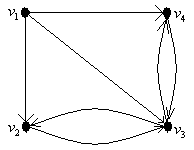
\includegraphics[width=5cm,height=4cm,keepaspectratio]{figures/image245.png}\par}\medskip

\par}\smallskip

1. 设图\(G\)如图 1 所示，

(1) 求\(G\)的邻接矩阵\(A\)；

(2) 求\(A^{(2)},A^{(3)},A^{(4)}\)，说明从\(v_{1}\)到\(v_{4}\)的长为\(2,3,4\)的路径各有几条；

(3) 求\(G\)的可达矩阵\(P\)；

(4) 求\(G\)的强连通分图。

2. 求群\(< N_{8}, +_{8} >\)的所有子群及由元素\(5\)确定的各子群的左陪集，其中\(N_{8} = \left\{ 0,1, \cdot \cdot \cdot ,7 \right\}\)，\(+_{8}\)是模\(8\)加法。

\pdfbookmark[1]{四、证明题（每小题10分，共40分）}{section166}

\par\medskip{\heiti

四、证明题（每小题 10 分，共 40 分）

\par}\smallskip

1. 证明布尔恒等式：\((a \ast b) \oplus (a' \ast c) \oplus (b' \ast c) = (a \ast b) \oplus c\)。

2. 设\(R\)为实数集合，\(+\)和\(\times\)为数的加法和乘法运算，对\(\forall a,b \in R\)，\(a*b = a + b + a \times b\)，

\begin{quote}
证明：\(< R, \ast >\)为独异点。
\end{quote}

3. 证明：若\((n,m)\)简单无向图\(G\)满足\(m > \frac{1}{2}(n - 1)(n - 2)\)，则图\(G\)是连通图。

4. 设\(< G, \ast >\)是一个群，\(a \in G\)；定义一个映射\(\left. f:G\rightarrow G \right.\)，使得对于\(\forall x \in G\)有\(f(x) = a \ast x \ast a^{- 1}\)；

证明：\(f\)是\(< G, \ast >\)

\par 原稿在末题此处截断。

\end{document}
